\documentclass[a4pper,11pt,onecolumn]{article}
\setlength\parindent{2em}
\usepackage{graphicx}
\graphicspath{ {./images/} }
\usepackage{mathtools}
\usepackage{indentfirst}
\usepackage{float}

\title{Web Searching and Mining Project}
\author{Professor : Ming Feng Tsai\\
        Student : Shu Hong Liu}

\begin{document}
\maketitle

\newpage
%abstract

\tableofcontents
\newpage
\listoffigures
\newpage

%section
\section{Introduction}
I used WT2G datasets which is part of WT10G from \textbf{TREC Web Corpus}.
Since 1992, a series of annual benchmarking evaluation exercises , called \textbf{TREC (Text REtrieval Conference)}, have launched in the USA. TREC experiments were designed to allow large-scale laboratory testing, compare the effectiveness and performance of different information retrieval techniques. TREC has become the standard in the IR field. So, here I used WT2G that is a smaller datasets from TREC.

In WT2G, we can find that there are 247491 documents and about 1,500,000 unique words. That is a big challenge for me, because I studied in Statistic and the number of documents is too big for me to do something. Fortunately, professor Tsai recommend Indri toolkit to do information retrieval more easily than I thought before.

\section{Method}
Here I am going to introduce the methods that I used.

\subsection{Vector Space Model}
In \textbf{vector space model}, the most important thing is \textbf{tf}, \textbf{idf} and \textbf{the measurement of distance}.\\
So, I used \textbf{Okapi} TF times IDF value and inner product similarity to calculate the distance between two vectors.

\[
    Okapi TF = \frac{tf}{tf + k1 \times ((1 - b) + b \times \frac{doclen}{avgdoclen})}
\]
At first, I set$$k1 = 2$$ and \[b = 0.75\] to see what is going on. The tuning parameter is important that will change result a lot.

\subsection{Language model with Laplace smoothing}
In language model, we have many smoothing methods. I used \textbf{Laplace smoothing} here, and \textbf{Jelinek-Mercer smoothing} will be the next method. In this method, I used maximum likelihood estimates with Laplace smoothing only, query likelihood.

I calculate each term's likelihood in each documents and multiply the term's likelihood which appears in query, and give each document a value. Because I assumed that the term's appearance is unigram, I used the multiplication. So, the document's value is bigger then it would be retrieved sooner.

The likelihood definitoin:
\[
    \rho_i = \frac{m_i + 1}{n + k}
\]
where m = term frequency\\
n = number of terms in document (doc length)\\
k = number of unique terms in corpus.

\subsection{Language model with Jelinek-Mercer smoothing}
In \textbf{Jenlinek-Mercer smoothing}, we still use term frequency, but we  need to consider a term appeared in one document and appeared in all documents. It is like local and global, we need to consider both situation. There will be a parameter to control which situation we care more. In this time, I take the parameter 0.8, that is to say I care the global situation more.

In this way, we don't be afraid of the query term didn't appear in some documents that get a term frequency equal to 0 to cause this document's value equal to 0.

\[
    \rho_i = \lambda \times P + (1 - \lambda) \times Q
\]
where P is the estimated probability from document (max likelihood = \[ \frac{m_i}{n}\])\\
and Q is the estimated probability from corpus (background probability = \[ \frac{cf}{terms in the corpus} \])

\section{Trials}
Before using methods that I mentioned above, I construct two indexes, (1) \textbf{without stemming}, and (2) \textbf{with stemming}. In each index, I used all of methods above, so there will be 6 runs.

\subsection{WT2G without stemming}
In this section, I constructed index without stemming, that is to say I barely did nothing. The reason I did nothing is that I wanted to know the baseline, just depend on the methods, how far that we can go.
Let's see the results.

\subsubsection{Vector Spcae Model}

    \begin{figure}[H]
    \centering
    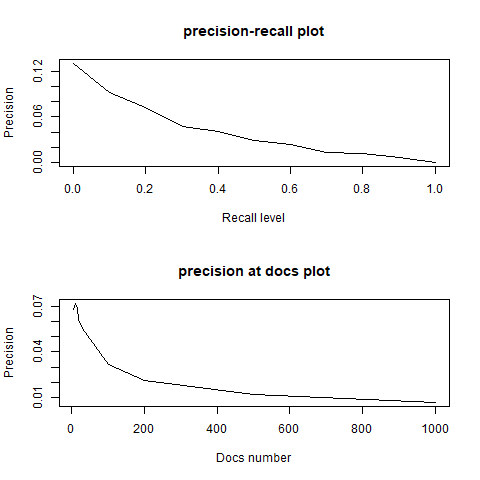
\includegraphics[scale = 0.6]{model2.png}
    \caption{Vector Space Model without stemming}
    \end{figure}
\subsubsection{Language model with Laplace smoothing}

    \begin{figure}[H]
    \caption{Language model with Laplace smoothing without stemming}
    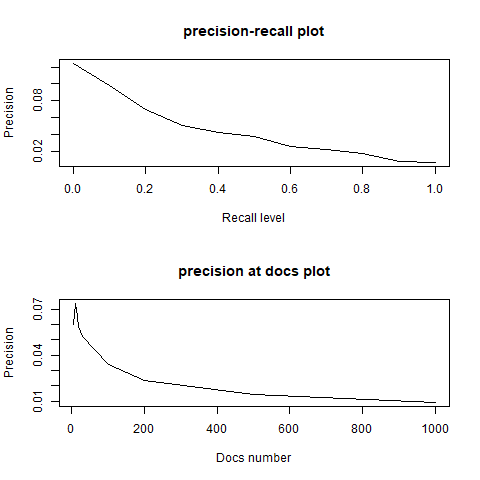
\includegraphics[scale = 0.6]{model4.png}
    \centering
    \end{figure}

\subsubsection{Language model with Jelinek-Mercer smoothing}

    \begin{figure}[H]
    \caption{language model with Jelinek-Mercer smoothing without stemming}
    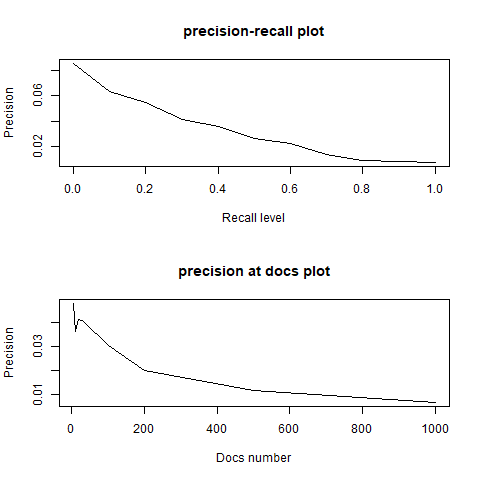
\includegraphics[scale = 0.6]{model6.png}
    \centering
    \end{figure}

\subsubsection{Combined}

    \begin{figure}[H]
    \caption{Three methods Precision - Recall plot without stemming}
    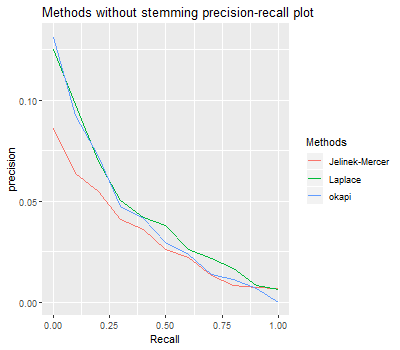
\includegraphics[scale = 0.6]{no_stemming_pr.png}
    \centering
    \end{figure}

    \begin{figure}[H]
    \caption{Three methods Precision at docs plot without stemming}
    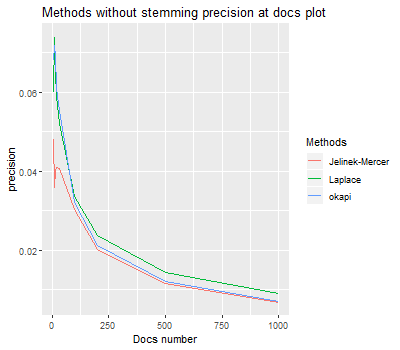
\includegraphics[scale = 0.6]{no_stemming_doc.png}
    \centering
    \end{figure}

\subsection{WT2G with stemming}

\subsubsection{Vector Spcae model}
\begin{figure}[H]
\caption{Vector Space Model with stemming}
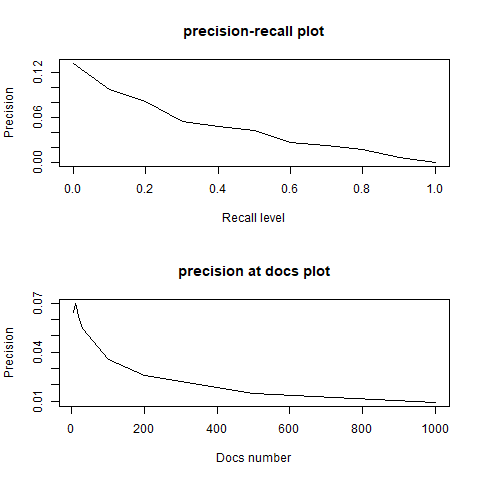
\includegraphics[scale = 0.6]{model1.png}
\centering
\end{figure}

\subsubsection{Language model with Laplace smoothing}
\begin{figure}[H]
\caption{Language model with Laplace smoothing with stemming}
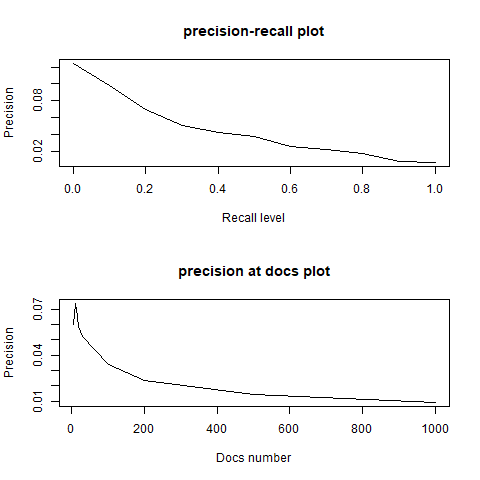
\includegraphics[scale = 0.6]{model3.png}
\centering
\end{figure}

\subsubsection{Language model with Jelinek-Mercer smoothing}
\begin{figure}[H]
\caption{Language model with Jelinek-Mercer smoothing with stemming}
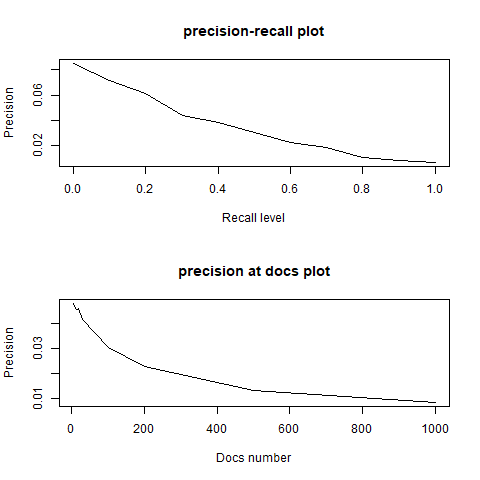
\includegraphics[scale = 0.6]{model5.png}
\centering
\end{figure}

\subsubsection{Combined}
\begin{figure}[H]
\caption{Three methods Precision-Recall plot with stemming}
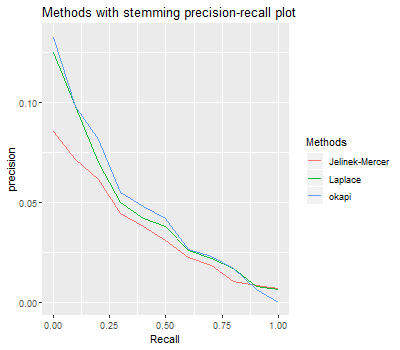
\includegraphics[scale = 0.6]{stemming_pr.png}
\centering
\end{figure}

\begin{figure}[H]
\caption{Three methods Precision at docs plot with stemming}
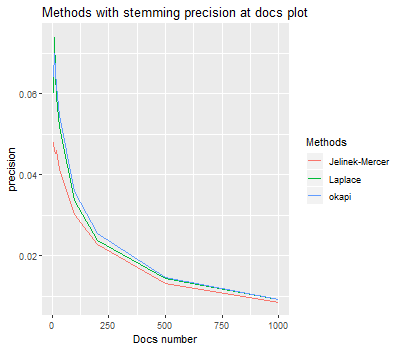
\includegraphics[scale = 0.6]{stemming_doc.png}
\centering
\end{figure}

\section{Idea}
In these trials , We can see that the results are bad enough. However, that means there's still room for improvement. I think that we can clean text by stemming, deleting stopwords, numbers and punctuation to get more accurate documents. Moreover, we can not only use queries' title from WT2G but also add nouns from queries' description and narrative which are used to describe more precisely about queries. Also, we can input qeury by query to find that in which query the method will work fine or in which query the method will work poor.

\subsection{Interesting}

\subsubsection{without stemming}

\subsubsection{with stemming}

\section{Conclusion}
In this project, I learned the toolkit Indri and some methods for information retrieval. In my opinion, I think that all of these methods are similar, and only the smoothing ways are a little different. I want to know the ultimate solution to solve language.\textbf{How did language start? Where languages come from? Why was language created?}A language's appearance was a singular point, but why and how? I want to find these answers.

\end{document}
